% !TEX root = handbook-physics.tex
% !TEX TS-program = pdflatex
% !TEX encoding = UTF-8 Unicode






\chapter{Electromagnetic Induction}
\label{ch-25}

\section{Basic Law of Electromagnetic Induction}
\label{sec-25.1}

\subsection{}\label{25.1.1} The \redem{phenomenon of electromagnetic induction} is the setting up of an \redem{induced electric field} in a conducting loop, or circuit, located in a varying magnetic field. The energy measure of this induced field is the \redem{electromotive force $\emf_{i}$ of electromagnetic induction}. If the loop is closed, the induced electric field causes ordered motion of electrons in the loop, i.e. a current, called the \redem{induced current}, is produced.

\subsection{}\label{25.1.2} \redem{Faraday's law of electromagnetic induction} states that the emf of electromagnetic induction in a loop, or circuit, is proportional to the rate of change of the magnetic flux \ssect{23.5.5} through the surface area bounded by this loop. Thus
\begin{align*}%
\emf_{i} & = - \dv{\Phi_{m}}{t} &&  \text{(in SI units),} \\
\emf_{i} & = - \frac{1}{c}\,\dv{\Phi_{m}}{t} &&  \text{(in Gaussian units).\sidenote{In all the formulas written in Gaussian units, $c$ is the electrodynamic constant.}}
\end{align*}



\ssect{23.2.2}

The cause of the change in the magnetic flux is unessential. It may be due to distortion of the loop or its motion in the external magnetic field or to any other reasons for the change in the magnetic field with time. When a closed conducting circuit (or loop) moves in a magnetic field, emf’s are induced in all of the parts of the loop that cut the lines of magnetic induction. The algebraic sum of these emf’s \ssect{25.1.3} is equal to the total emf of the loop. The work that must be done to move a closed loop, or circuit, in a magnetic field is equal to the work of the current induced in the loop.

In calculating $\Phi_{m}$ and $\emf_{i}$ the directions around the loop \ssect{21.3.2} and of the outward normal $\vu{n}$ (\ssect{23.5.5} and \ssect{23.5.8}) are to be coordinated so that from the head of vector n the direction around the circuit (or loop) is seen to be counterclockwise. If a closed circuit consists of $N$ turns connected in series (for example, the solenoid in Section \ssect{23.3.7}), then the magnetic flux $\Phi_{m}$ in Faraday’s law is to be replaced by the flux, or magnetic, linkage $\Psi$ of the circuit (\ssect{23.6.5}:
\begin{align*}%
\emf_{i} & = - \dv{\Psi}{t} &&  \text{(in SI units),} \\
\emf_{i} & = - \frac{1}{c}\,\dv{\Psi}{t} &&  \text{(in Gaussian units)}.
\end{align*}

\subsection{}\label{25.1.3} The emf of electromagnetic induction in a loop (or circuit) is said to be positive if the magnetic moment vector $\vb{p}_{m}$ of the corresponding induction current \ssect{23.3.4} makes an acute angle with the lines of magnetic induction of the field that induces this current. Otherwise, $\emf_{i}$ is said to be negative. In \figr{fig-25-01}~\drkgry{(a)}, the emf $\emf_{i} < 0$, whereas in \figr{fig-25-01}~\drkgry{(b)}, $\emf_{i} > 0$. 

\begin{figure}%[-2cm]
\centering
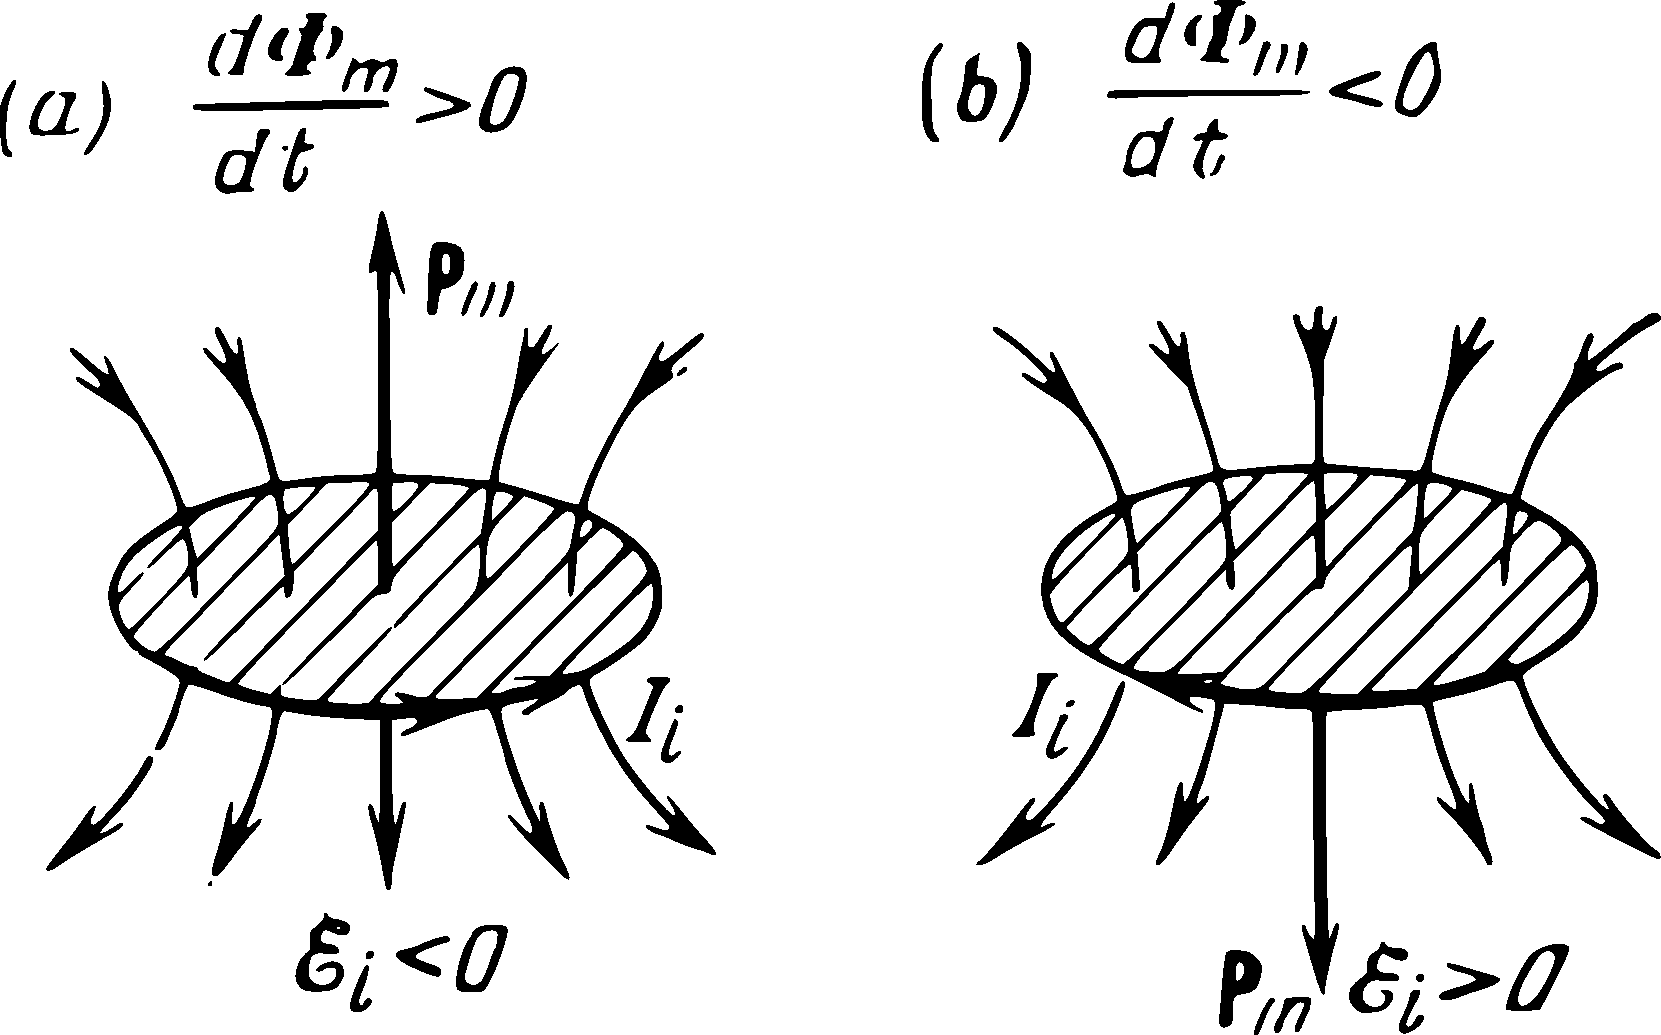
\includegraphics[width=0.8\textwidth]{figs/ch-25/fig-25-01.pdf}
\sidecaption{Determining the direction of emf generated.\label{fig-25-01}}
\end{figure}


\subsection{}\label{25.1.4} The minus sign in the formula for  complies with the \redem{Lenz law}, which states that upon any change in the magnetic flux through a surface bounded by a closed loop, the current induced in the loop is always of a direction in which the magnetic field set up by the induced current opposes the change in the magnetic flux that induced the current.

\subsection{}\label{25.1.5} An emf of electromagnetic induction is developed in a part of a conductor which, in its motion, cuts lines of induction of a magnetic field \ssect{23.1.3}. In the case illustrated in Fig. 25.2, the conduction electrons of the metal \ssect{20.3.1} are subject to the Lorentz force \ssect{24.1.1}. Thus $\vb{F}_{L} = — e [(\vb{v} + \vb{v}') \cross \vb{B}]$, where $\vb{v}$ is the velocity of the part $AC$ of the conductor in the magnetic field, whose induction vector $\vb{B}$ is perpendicular to the plane passing through the part of the conductor and the velocity vector of its motion. The electrons travel orderly along the conductor at the velocity $\vb{v}'$ by the action of the component of the Lorentz force tangent to the conductor in the direction from $A$ to $C$. The motion of the electrons ceases when the electrostatic field set up in the conductor and acting on the electrons with the force $e\vb{E}$ counterbalances the Lorentz force.
\begin{figure}%[-2cm]
\centering
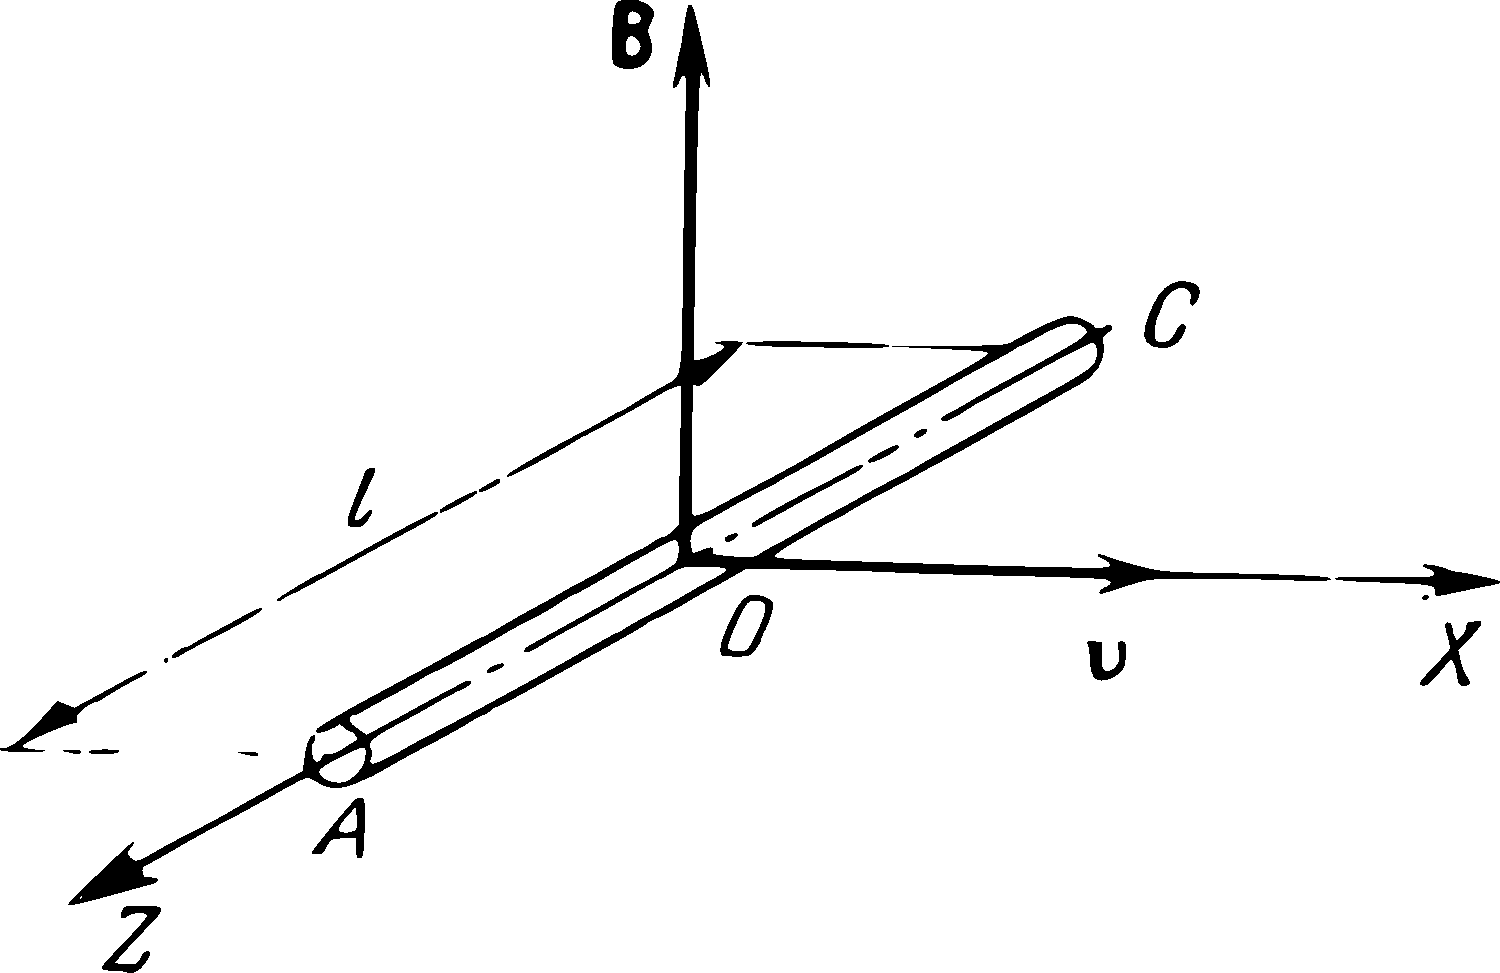
\includegraphics[width=0.8\textwidth]{figs/ch-25/fig-25-02.pdf}
\sidecaption{An emf of electromagnetic induction is developed in a part of a conductor which, in its motion, cuts lines of induction of a magnetic field.\label{fig-25-02}}
\end{figure}


According to Ohm’s law for an open circuit (at $I = 0$) \ssect{21.2.5}, the equilibrium potential difference $\Delta V = V_{A} - V_{C}$ between points $A$ and $C$ that is established at $\vb{v}' = 0$ is equal to
\begin{equation*}%
\Delta V = V_{A} - V_{C} = - \emf_{i},
\end{equation*}
where $\emf_{i}$ is the electromotive force of induction, because there are no sources of electrical energy in part $AC$ of the conductor. The emf of electromagnetic induction in a piece of conductor of length $l$, moving at the velocity $v$, is
\begin{align*}%
\emf_{i} & = - Bvl, \qor \\
\emf_{i} & = - \dv{\Phi_{m}}{t} \,\, \text{(in SI units)}, 
\end{align*}

where $\dv*{\Phi_{m}}{t}$ is the ratio of the magnetic flux through the surface generated by the conductor in its motion during an infinitesimal length of time to the value $\dd t$ of this length of time or, in other words, the velocity at which the conductor cuts the lines of induction of the magnetic field (cf. Section \ssect{25.1.2}). 

\subsection{}\label{25.1.6} The phenomenon of electromagnetic induction in stationary closed conducting circuits, located in an external varying magnetic field, cannot be explained by means of the Lorentz force, which has no effect on fixed charges \ssect{24.1.1}.

The phenomenon of electromagnetic induction in stationary conductors is due to the fact that the varying magnetic field excites a rotational electric field. The circulation of the strength vector of this field along the closed path $L$ of the conductor \ssect{16.1.4} is the emf of electromagnetic induction. Thus
\begin{align*}%
\emf_{i} & = \oint \vb{E}\, \dd \vb{l} = \dv{\Phi_{m}}{t} &&  \text{(in SI units),} \\
\emf_{i} & = \oint \vb{E}\, \dd \vb{l} = \dv{\Phi_{m}}{t} \frac{1}{c}\,\dv{\Psi}{t} &&  \text{(in Gaussian units)}.
\end{align*}
where the partial derivative $\dv*{\Phi_{m}}{t}$ takes into account the dependence of the magnetic induction flux only on time. The choice of the direction of normal $\vu{n}$ in calculating the magnetic flux is discussed in Section \ssect{25.1.2}.

\subsection{}\label{25.1.7} The magnitude $q$ of the electric charge passing through the cross section of the wire of the turn in which the current is induced is
\begin{align*}%
q & = \frac{\Phi_{m}' - \Phi_{m}''}{R} && \text{(in SI units),} \\
q & = \frac{1}{c} \, \frac{\Phi_{m}' - \Phi_{m}''}{R}  &&  \text{(in Gaussian units)},
\end{align*}
where $\Phi_{m}'$ and $\Phi_{m}''$ are the values of the magnetic flux through the area of the turn in its initial and final positions, and $R$ is the electrical resistance of the turn.


\section{Phenomenon of Self-Induction}
\label{sec-25.2}

\subsection{}\label{25.2.1} Self-induction is the production of an induced electric field in a circuit as a result of the variations of current in the same circuit. The energy characteristic of the induced field is the emf of self-induction

\subsection{}\label{25.2.2} The intrinsicmagnetic field of the current in the circuit produces the magnetic flux Oms through the surface S bounded by the current-carrying loop. Thus
(hms=  tindS,,
S
where Bn is the projection of the induction vector B of the mag­ netic field \ssect{23.1.2} on the normal n to the element of surface dS. The quantity <Pms is called the magnetic flux of self-induction of the loop. Making use of the Biot-Savart-Laplace law \ssect{23.2.2}, Oms can be calculated for the case in which the loop is in a nonferromagnetic medium \ssect{26.5.2}:
J’ms= [dSI)f[dlrj„ (inSIunits), SL
ms = -— /  dS  ——[c?l r]n (in Gaussian units), SL

or
 ms= LI (in SI units),
1
Oms= —LI (in Gaussian units), c
where L is called the self-inductance of the loop and is deter­ mined by the formulas
L =  d S () — [ i l r ] n ( i n S I u n i t s ) , 5? L
L= dS()—[dr]n(inGaussianunits). SL
Here p0is the magnetic constant in SI units \ssect{23.2.2}, fxr is the relative magnetic permeability of the medium, r is the radius vector from element dl of the loop to element dS of surface S, bounded by the loop, and subscript n indicates the projection on the normal to the element dS.

\subsection{}\label{25.2.3} The self-inductance L of the loop is numerically equal to the self-induction flux at a current of I = 1 A (in SI units) or I = c (in Gaussian units). Self-inductance L depends only upon the geometric shape and dimensions of the loop, as well as on the magnetic properties of the medium it is located in. The self-inductance of a sufficiently long solenoid \ssect{23.4.8} is
L= v-mS=|j0!1[.re2I/(inSIunits),
L =  —4jt|xrre3F (in Gaussian units).
where I and S are the length and cross-sectional area of the so­ lenoid, N is the total number of turns, n = N/l is the number of turns per unit length, and V = SI is the volume of the so­ lenoid.

\subsection{}\label{25.2.4} The expression for the emf of self-induction follows from Faraday’s law \ssect{25.1.2}:
« s=-T=F(i/)(inSIunits),
'Ss=---- = — ---(LI) (in Gaussian units).
For a rigid (undeformable) loop in a nonferromagnetic medium (26.5.2) L = const. Hence
rtT
—-L-jj- (inSIunits),
L dl
<sP= ---c2~df Gaussian units).

\subsection{}\label{25.2.5} The electromotive force of self-induction causes a self-induction current to flow in the loop. According to the Lenz
Fig. 25.3 Fig. 25.4
law \ssect{25.1.4}, this current counteracts the change in the main current in the circuit, impeding its increase or decrease. The self-inductance of the loop \ssect{25.2.3} is a measure of its inertia to changes of the current.

\subsection{}\label{25.2.6} The law for the change of the current in closing and open­ ing a circuit, i.e. with a nonsteady state in the circuit, is
/=v -Ri/t+ f a-«-Bn
where /0 is the current at the initial instant of time (f = 0), R is the electrical resistance of the circuit, L is its self-induc­ tance, and  is the algebraic sum of the emf’s of the sources of electrical energy connected into the circuit \ssect{21.2.2}.

When the source of emf is switched in there is no initial current in the circuit (/0= 0):
/=-| (i- e-R).
The current in the circuit increases from zero to the value lR, corresponding to that of the constant current. The higher the
Sw
ratio R/L (Fig. 25.3), the more rapidly the current increases. When the source of emf is switched off,  — 0:
I= I0e-Rt/L.
The current decreases exponentially from the initial value /0. The higher the ratio R/L, the more rapidly the current decreases (Fig. 25.4).

\section{Mutual Induction}
\label{sec-25.3}

\subsection{}\label{25.3.1} An emf is induced in all conductors in the vicinity of a circuit in which the current varies. This phenomenon is called mutual induction. Upon a change in the current I x in circuit 1 (Fig. 25.5), for example, an emf 2i mutual induction is in­ duced in circuit 2. It equals
21= — (ln SI UnitS>- ---(in Gaussian units),
where m21 is the magnetic flux through the surface bounded by the second circuit. This flux is due to the magnetic field set up by the current in the first circuit (magnetic flux of mutual induction).

\subsection{}\label{25.3.2} By analogy with section \ssect{25.2.2}, the magnetic flux Om21 is proportional to the current /x. Thus
<J>m2i==Af2i/i (in SI units), 1
<Dm21 = “ Af2i-/i (in Gaussian units),
where M2i is called the mutual inductance of the second and first circuits. The quantity M21 depends upon the shape, di­ mensions and relative arrangement of the circuits, as well as the relative magnetic permeability of the medium surround­ ing them. The magnetic flux (Dmi2through the surface bounded by the first circuit is due to the magnetic field set up by current 12 in the second circuit. Thus
(I)mi2=  i 22 (in SI units),
1
(Dm12 = — M 12T2 (in Gaussian units),
where M12 is the mutual inductance of the first and second circuits.
If the circuits are in a nonferromagnetic medium \ssect{26.5.2}, then M21= M12. F6r ferromagnetic media M21 and M12 are not equal and depend, in addition to the above-mentioned factors, on the currents in the two circuits and the way in which they vary.

\subsection{}\label{25.3.3} The expressions for the emf of mutual induction, under the condition that M21 and M12 are both constant values, are
jr
21= —M2i -—- (in SI units),
21= ----M2i ‘S 12= — M 12
(in Gaussian units),
(in SI units),
A  1 2 = --- (in
flT
Gaussian units).

An example of the application of mutual induction is the principle of the transformer which serves to raise or lower the volt­ age of alternating current.


\section[Energy of a Magnetic Field]{Energy of a Magnetic Field Set up by an Electric Current} *
\label{sec-25.4}

\subsection{}\label{25.4.1} To produce an electric current in a closed circuit (or loop) and to increase this current from zero to I it is necessary to do work W to overcome the emf of self-induction that impedes the increase in current \ssect{25.2.6}. Thus
W=-~ =~ (inSIunits),
W=-t = —L (in Gaussian units),
where Oms is the magnetic flux of self-induction of the loop \ssect{25.2.2} and L is the self-inductance of the loop \ssect{25.2.2}. According to the energy conservation law, W determines the intrinsic energy Em of current I in a circuit. Thus
LI2
Z?m= — (in SI units),
(in Gaussian units).

\subsection{}\label{25.4.2} Increasing together with the current in a circuit is the magnetic field set up by this current. Hence, the intrinsic energy of a current is dealt with as energy of this magnetic field. In a long solenoid \ssect{23.3.8}, for instance, having a uniform magnet­ ic field \ssect{23.1.2},
1
Em= --ii0ixrn2I2V (in SI units),
Em= 2nn2I2V (in Gaussian units),
* It is assumed in this section that the conductors carrying currents are in a nonferromagnetic, homogeneous and iso­ tropic medium.

where V is the volume of the solenoid, n is the number of turns per unit length, j l0i is the magnetic constant \ssect{23.2.2}, and p,r is the relative permeability of the medium.

\subsection{}\label{25.4.3} The volume energy density Em of a magnetic field is the energy per unit volume of the field. Thus
d dEm m dV*
For a uniform magnetic field \ssect{23.1.3}, Em = Em/V.
The volume energy density of any, including a nonuniform magnetic field, is expressed by the formula
<= -|BH=-MirIP=2- (inSIunits),
nd BH iTm 1 B* „
EL= —— = —— =-5------(in Gaussian units).
m 8n 8ji 8n p,r v J
Here B and H are'the magnitudes of the vectors of magnetic induction \ssect{23.1.2} and strength \ssect{23.2.3} at the point being considered in the magnetic field. The remaining notation is defined in Sect. \ssect{25.4.2}.

\subsection{}\label{25.4.4} The energy of a magnetic field, localized in the volume V is
Em— j dV (in SI units),
V
Em=  dV (in Gaussian units). v

\subsection{}\label{25.4.5} If the magnetic field is set up by an arbitrary system of n circuits, or loops, with the currents 71? /2, /3, . . ., I n, the energy of the field can be expressed by the formula of Sect. \ssect{25.4.4}, in which B and H are understood to be the magnitudes of vectors B and H of the resultant magnetic field, in accordance
 334
with the principle of superposition of fields \ssect{15.2.2}. Moreover, the energy of the magnetic field in this case is
n
hih
where Omh is the total magnetic flux linked to the Tcth loop \ssect{23.6.5}. In calculating this flux, the normal nk to the surface bounded by the loop is such that from the head of vector nk the current is seen to be counterclockwise. The magnetic flux
equals
mk—msh+ ®mmhi
where ® msfc is the magnetic flux of self-induction of the fcth loop \ssect{25.2.2} and Ommft is the magnetic flux of its mutual in­ duction, produced by all the other loops carrying current \ssect{25.3.1}. Hence the energy Em of the magnetic field is equal to
k=i i=[(l=£k)
The first term is the sum of the intrinsic energies of all the cur­ rents \ssect{25.4.1}. The second term is called the mutual energy of the currents. Here Mki is the mutual inductance of the Zcth and Zth loops, or circuits, \ssect{25.3.2} with the currents and 11.


